% fig:inverse_shading — regenerated from our own Hypersim data by
% tests/viz/build_inverse_shading_figure.py. The panels are raster (they are images); the
% three distributions are drawn here as pgfplots so they are vector, sharp at any zoom, and
% set in the document's own fonts. Data: chapters/data/shading_hist_*.dat
\begin{figure}[t!]
  \centering
  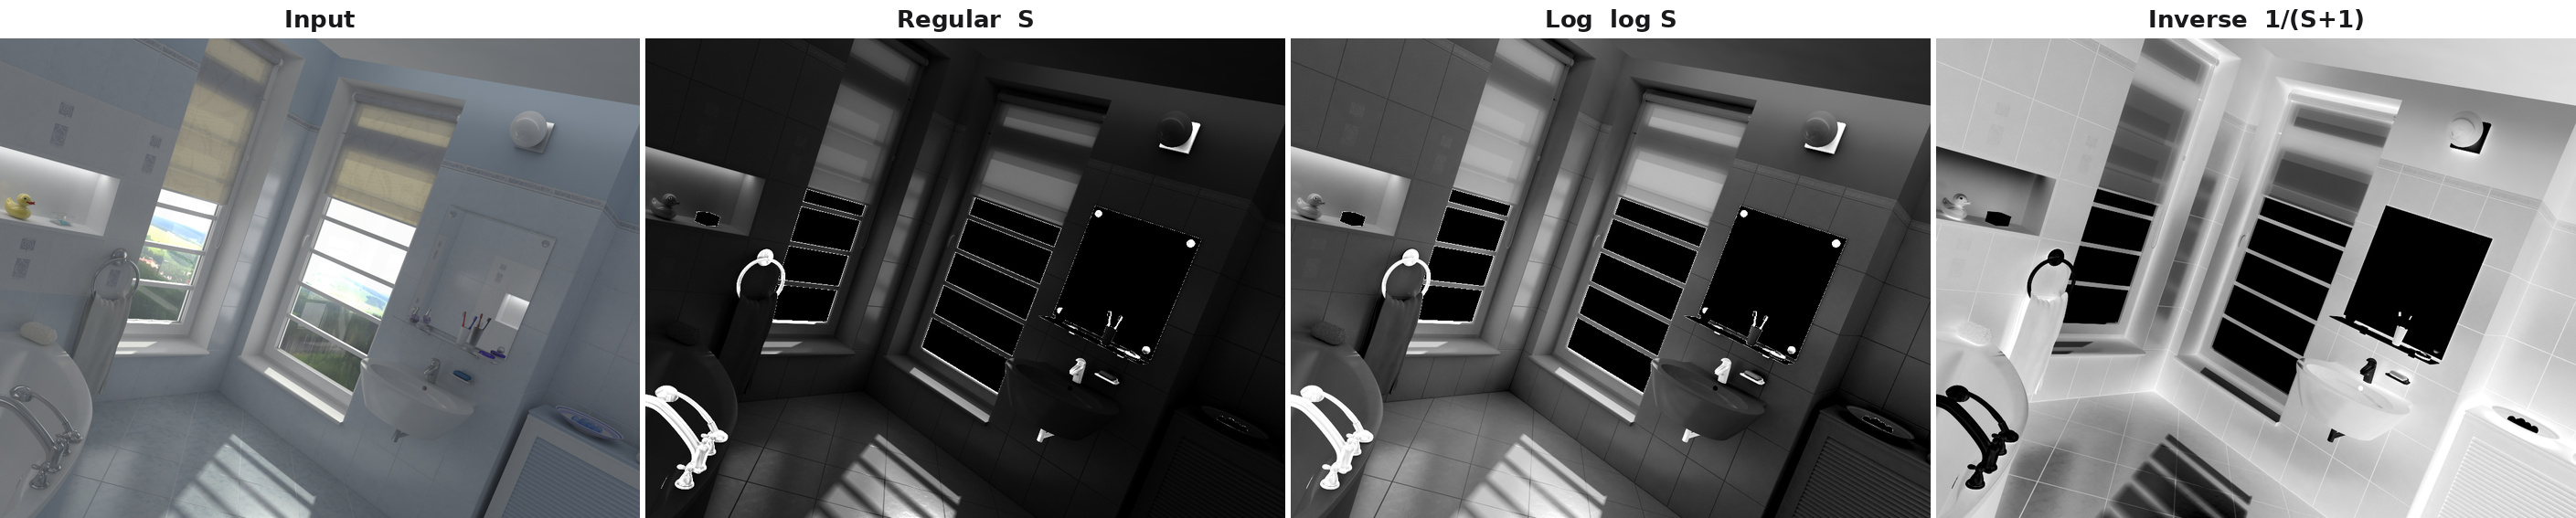
\includegraphics[width=\textwidth]{images/inverse_shading/panels.jpg}\\[6pt]
  \pgfplotsset{
    shadinghist/.style={
      width=0.35\textwidth, height=3.6cm,
      ybar, bar width=1.1pt,
      ymin=0, ymax=1.10,
      axis lines=left,
      axis line style={gray!55},
      tick label style={font=\scriptsize},
      xlabel style={font=\scriptsize, yshift=2pt},
      ylabel style={font=\scriptsize},
      ytick=\empty,
      minor tick num=0,
      xtick align=outside,
      grid=none,
      title style={font=\scriptsize, yshift=-2pt},
      every axis plot/.append style={
        fill=blue!50!cyan, draw=none},
    }}
  \begin{tikzpicture}
    \begin{axis}[shadinghist, xlabel={$S$ \, (linear)}, ylabel={density},
                 xmin=-0.15, xmax=5.4, xtick={0,1,2,3,4,5},
                 title={Regular: mass collapses at $0$}]
      \addplot table[x=x, y=y] {chapters/data/shading_hist_regular.dat};
    \end{axis}
  \end{tikzpicture}\hfill
  \begin{tikzpicture}
    \begin{axis}[shadinghist, xlabel={$\log S$},
                 xmin=-1.75, xmax=1.8, xtick={-1.5,-0.5,0.5,1.5},
                 title={Log: balanced but unbounded}]
      \addplot table[x=x, y=y] {chapters/data/shading_hist_log.dat};
    \end{axis}
  \end{tikzpicture}\hfill
  \begin{tikzpicture}
    \begin{axis}[shadinghist, xlabel={$1/(S+1)$},
                 xmin=-0.03, xmax=1.03, xtick={0,0.25,0.5,0.75,1},
                 title={Inverse: spread across $[0,1]$}]
      \addplot table[x=x, y=y] {chapters/data/shading_hist_inverse.dat};
    \end{axis}
  \end{tikzpicture}
  \caption[Inverse-shading parameterisation and target distributions.]{%
    Why shading is regressed in the inverse domain. Shading is derived from Hypersim ground
    truth as $S = \mathbf{I} / \mathbf{A}$ and shown in three representations, with the
    distribution of its values beneath each.
    Linear shading is dominated by a small number of very bright pixels. It runs to
    $5.3$ on this frame, so almost all of the mass collapses into the first bin and a
    regressor spends its capacity on outliers.
    Log shading balances the distribution but has no bounded range, so it cannot be produced
    by a saturating output nonlinearity.
    Inverse shading, $1/(S+1)$, is confined to $[0,1]$ \emph{by construction} and spreads
    across it, which makes it a well-conditioned target for a sigmoid head: this is the
    representation our shading branch predicts (\secref{sec:physics}), following
    \mycitetext{careaga23ordinal}. The physics losses that need real light intensity operate
    on the linear $\mathbf{S}_d$ recovered from it.
  }
  \label{fig:inverse_shading}
\end{figure}
